\documentclass[a4paper,8pt]{extarticle}

%%% Работа с русским языком
\usepackage{cmap}					% поиск в PDF
\usepackage{mathtext} 				% русские буквы в формулах
\usepackage[T2A]{fontenc}			% кодировка
\usepackage[utf8]{inputenc}			% кодировка исходного текста
\usepackage[english,russian]{babel}	% локализация и переносы

%%% Дополнительная работа с математикой
\usepackage{amsmath,amsfonts,amssymb,amsthm,mathtools} % AMS
\usepackage{icomma}
\usepackage{physics}
\usepackage{multicol}
\usepackage{bm}
\usepackage{mathrsfs}
\usepackage{verbatim}

%%% Номера формул
%\mathtoolsset{showonlyrefs=true} 
%\usepackage{leqno} 

%%% Свои команды
\DeclareMathOperator{\sgn}{sgn}

\usepackage{csquotes} 
\usepackage[backend=biber,style=authoryear,language=auto]{biblatex}
\addbibresource{source.bib}


%%% Работа с графикой
\usepackage{graphicx}
\graphicspath{{images/}}  
\setlength\fboxsep{3pt} 
\setlength\fboxrule{1pt} 
\usepackage{wrapfig} 
\usepackage{tikz}
\usepackage{pgfplots}
\usepackage{pgfplotstable}
\usepgfplotslibrary{polar}
\pgfplotsset{compat=1.18} 

%%% Работа с таблицами
\usepackage{array,tabularx,tabulary,booktabs}
\usepackage{longtable}  
\usepackage{multirow} 
\usepackage{caption2}[2008/03/29]
\usepackage{soul} 

%%% Теоремы
\theoremstyle{plain} 
\newtheorem{theorem}{Th}[section]
\newtheorem{proposition}[theorem]{Proposition}
 
\theoremstyle{definition} 
\newtheorem{corollary}{Corollary}[theorem]
\newtheorem{problem}{Problem}[section]
\newtheorem{definition}{Def}[section]
 
\theoremstyle{remark} 
\newtheorem*{nonum}{Solution}

%%% Программирование
\usepackage{etoolbox} 

%%% Гиперссылки
\usepackage{hyperref}

\usetikzlibrary{knots}
\usepackage{tcolorbox}

%%% Страница
\usepackage{geometry} 
	\geometry{top=20mm, bottom=20mm, left=15mm, right=20mm}

\usepackage{fancyhdr} 
 	\pagestyle{fancy}
 	\renewcommand{\headrulewidth}{1pt}  
    \rhead{\today}
    \lhead{Новохатний Артем, Цыганкова Екатерина, Мифтахов Эльдар}

\usepackage{setspace} 

\usepackage{lastpage} 


\begin{document}
\begin{center}
    \Huge Полиномы Хованова
\end{center}
\begin{multicols}{2}
\subsection*{Глобальная задача:}
Найти инварианты узлов, которые бы позволили различать их между собой. Привести эффективный алгоритм их вычисления.

\columnbreak
\subsection*{Локальная задача:}
...
\end{multicols}

\hrule

\begin{multicols}{2}
    \section{Пара слов о скобке Кауфмана}
    В предыдущий раз было предложено рассмотреть следующую конструкцию
    построения скобки Кауфмана:

    \begin{equation}
    \left\langle 
    \begin{minipage}{0.06\linewidth}
    \resizebox{\linewidth}{!}{\begin{tikzpicture}
\begin{knot}[
consider self intersections,
clip width=5,
]
\strand[line width=3pt, black]
(-1, -1) to[out=45,in=-135,looseness=1] (1, 1);
\strand[line width=3pt, black]
(-1, 1) to[out=-45,in=135,looseness=1] (1, -1);
\end{knot}
\end{tikzpicture}}
    \end{minipage} \right\rangle = 
    a \cdot \left\langle 
    \begin{minipage}{0.06\linewidth}
    \resizebox{\linewidth}{!}{\begin{tikzpicture}
\begin{knot}[
consider self intersections,
clip width=5,
]
\strand[line width=3pt, black]
(-1, -1) to[out=60,in=-90,looseness=1]
(-0.5, 0) to[out=90,in=-60,looseness=1] (-1, 1);
\strand[line width=3pt, black]
(1, -1) to[out=120,in=-90,looseness=1]
(0.5, 0) to[out=90,in=-120,looseness=1] (1, 1);
\end{knot}
\end{tikzpicture}}
    \end{minipage} \right\rangle + b \cdot 
    \left\langle 
    \begin{minipage}{0.06\linewidth}
    \resizebox{\linewidth}{!}{\begin{tikzpicture}
\begin{knot}[
consider self intersections,
clip width=5,
]
\strand[line width=3pt, black]
(-1, -1) to[out=30,in=180,looseness=1]
(0, -0.5) to[out=0,in=150,looseness=1] (1, -1);
\strand[line width=3pt, black]
(-1, 1) to[out=-30,in=180,looseness=1]
(0, 0.5) to[out=0,in=-150,looseness=1] (1, 1);
\end{knot}
\end{tikzpicture}}
    \end{minipage} \right\rangle
    \label{eq:skein-kaufman}
    \end{equation}

    \begin{equation}
    \left\langle 
    \begin{minipage}{0.06\linewidth}
    \resizebox{\linewidth}{!}{\begin{tikzpicture}
\begin{knot}
\strand[line width=3pt, black] 
(0,0) circle[radius=1cm];
\end{knot}
\end{tikzpicture}}
    \end{minipage} \right\rangle = c
    \end{equation}

    \begin{equation}
    \langle L_1 \cup L_2\rangle = d \cdot \langle L_1\rangle \langle L_2 \rangle
    \end{equation}

    И подобрать коэффициенты $a, b, c, d$ исходя из инваринатности
    относительно всех ходов Рейдемейстера.

    Получаем три решения:

    \begin{equation}
        a=b=-1, \ \ cd=-2
        \label{eq:sol-kauf-1}
    \end{equation}

    \begin{equation}
        a = e^{\pm \frac{i \pi}{3}}, \ \ b = e^{\mp \frac{i \pi}{3}},
         \ \ cd=1
         \label{eq:sol-kauf-2}
    \end{equation}

    Данные полиномы оказываются слабыми: \eqref{eq:sol-kauf-1}
    различает только количество компонент зацепления, а \eqref{eq:sol-kauf-2}
    даёт одинаковые результаты для кружка, трилистника и зацепления Хопфа.

    \section{Переход от полинома Джонса к полиному Хованова. Гиперкуб, морфизмы}

    Напомним, что под отрицательным сглаживанием (или 0-сглаживанием) будем понимать первое разрешение в
    \eqref{eq:skein-kaufman}, а положительным (или 1-сглаживанием) - второе. Пользуясь этой
    терминологией мы построили ненормализованный полином Джонса в виде
    статсуммы:

    \begin{equation}
    \langle L \rangle=\sum_\alpha (-q)^{r} (q + q^{-1})^k
    \label{eq:statsum}
    \end{equation}

    Основная идея дальнейших рассуждений - заменить полиномы на вектроные пространства
    нужной градуировки, получив тем самым уже объект гомологической
    алгебры.
    
    Для дальнейших рассуждений полезно ориантироваться на Рис.
    \ref{fig:bar-natan-2}, а также ввести следующие определения:

    \begin{definition}
        Квантовой размерностью градуированного векторного пространства $W = \bigoplus_m W_m$
        будем называть \\ $q\dim W = \sum_m q^m \dim W_m$
        \label{def:qdim}
    \end{definition}

    \begin{definition}
        Будем называть $\cdot \{l\}$ операцией сдвига степени на
        градуированных векторных пространствах, если $W_m\{l\} = W_{m+l}$.
        Нам важно, что тогда $q\dim W\{l\} = q^l \cdot q\dim W$
    \end{definition}

    Определение \ref{def:qdim} даёт нам возможность ассоциировать
    с кружочком градуированное простанство $V = V_{+1} \oplus V_{-1}$:

    \begin{equation}
        \left\langle 
        \begin{minipage}{0.04\linewidth}
        \resizebox{\linewidth}{!}{\begin{tikzpicture}
\begin{knot}
\strand[line width=3pt, black] 
(0,0) circle[radius=1cm];
\end{knot}
\end{tikzpicture}}
        \end{minipage} \right\rangle = 
        q\dim V = q + q^{-1}
    \end{equation}

    Пусть $\chi$ - множество всех перекрестков, $|\chi| = n$. Тогда вектора $\alpha \in
    \{0,1\}^\chi$ естественным образом кодируют все разрешения. При
    потсроении гиперкуба мы начинаем с нулевого вектора (т.е. все
    перекрестки сглажены отрицательно). В следующем слое находятся
    вектора, отличающиеся от нулевого заменой одного из нулей на
    единицу. Будем продолжать по аналогии и у нас получатся $2^n$
    вершин, каждая из которых соединена с другими ровно $n-1$ ребром - 
    именно поэтому будем называть получившуюся конструкцию гиперкубом.

    Если бы в каждой вершине мы посчитали бы скобку Кауфмана
    и сложили результаты с учётом знаков, мы получили бы в точности
    \eqref{eq:statsum} и опять полином Джонса. Но теперь, каждой
    вершине мы припишем векторное пространство $V_\alpha = V^{\otimes k}\{r\}$,
    где $k$ - количество кружочков, $r=|\alpha|$ - количество положительных
    сглаживаний.

    Теперь будем двигаться в сторону построения цепного комплекса.
    В качестве цепных групп возьмем $[\![ L ]\!]^r = \bigoplus_{\alpha: r=|\alpha|} V_\alpha$


    \columnbreak
\end{multicols}

\begin{figure}[h]
  \centering
  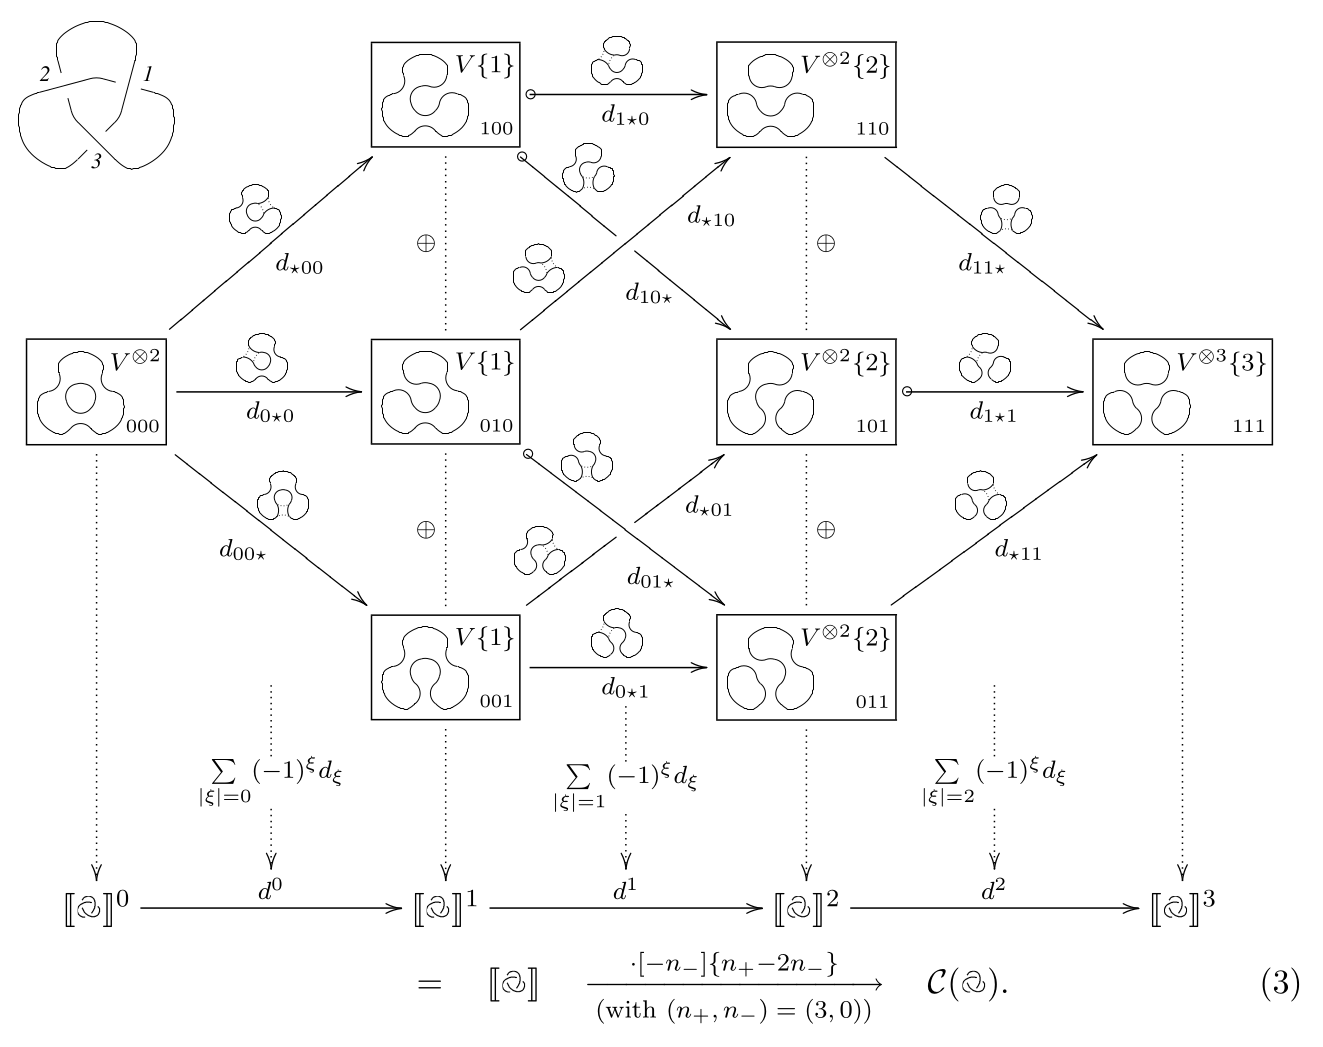
\includegraphics[width=0.8\linewidth]{../img/bar-natan-2.png}
  \caption{Пояснение к построению полинома Хованова \parencite{bar-natan}}
  \label{fig:bar-natan-2}
\end{figure}

\printbibliography
\end{document}
